\chapter*{Capítulo 1 \vspace{0.5cm} \break Fundamentos teóricos}
\setcounter{chapter}{1}
\addcontentsline{toc}{chapter}{Capítulo 1: Fundamentos teóricos}

En el presente capítulo se encuentran los fundamentos teóricos del nuevo sistema que se pretende desarrollar. Comprende un análisis de los sistemas de capacitación presencial y automatizados, reflejando un estudio de las preguntas más utilizadas, así como los colores y métodos de evaluación. Se introduce el término de sistema experto, con sus características y ventajas. Se detallan las funcionalidades del Sistema Generador de Bases de Conocimiento (SGBC) y se profundiza el trabajo con el sistema SECPROIT, finalizando con las conclusiones del capítulo.

%%%%%%%%%%%%%%%%%%%%%%%%%%%%%%%%%%%%%

\section{Sistemas de capacitación laboral}
La capacitación laboral es un método aplicado por las empresas para que su personal adquiera nuevos conocimientos profesionales. Por lo general, se produce ante un ascenso o incorporación, aunque no son los únicos motivos. Busca perfeccionar al colaborador en su puesto laboral, en función de las necesidades de su empresa. Es un proceso estructurado con metas bien definidas. Surge en el mundo como respuesta a la necesidad de mejorar permanentemente la calidad y formación de recursos humanos. Lo ideal es que se desarrolle de forma continua, ya que la constante formación del personal deriva en resultados positivos tanto para el grupo de trabajo como para la organización en la que se realiza \cite{Denby2010}.

\subsection{Características de un sistema de capacitación}
Un sistema de capacitación puede ofrecer diferentes aplicaciones en función del modelo de negocio que utilice. Su versatilidad permite adaptarse a las necesidades particulares de cada sector. Sin embargo, según \cite{Paez2022}, la mayoría de las capacitaciones contienen las siguientes características:

\begin{itemize}
\item Son capaces de gestionar los distintos cursos impartidos, la asistencia y la inversión en formación de la empresa
\item Asignan a los empleados que deberán asistir y a los profesionales responsables de analizar sus resultados
\item Detectan las carencias formativas del personal antes de que influyan en el desarrollo del trabajo
\item Clasifican las distintas actividades formativas en base a su categoría y catálogo
\item Registran y consultan el progreso del aprendizaje de los empleados en tiempo real
\end{itemize}

\subsection{Importancia de una buena capacitación}
La capacitación laboral juega un papel primordial para el logro de tareas y proyectos, dado que es el proceso mediante el cual los trabajadores adquieren conocimientos, herramientas, habilidades y actitudes para interactuar de forma correcta y segura en el entorno laboral. Entre los principales beneficios que aporta, según \cite{RogelioE.Martinez2002}, se destacan:

\begin{itemize}
\item Calidad y mejora en el resultado de las tareas
\item Reducción en tiempos de trabajo y supervisión
\item Solución de problemas con diferentes visiones
\item Sensibilización ante nuevos retos
\item Desarrollo ético y motivación del personal
\item Seguridad y autoestima en los trabajadores
\item Mayor especialización
\end{itemize}

\subsection{Proceso de evaluación en una capacitación}
La evaluación de una capacitación no puede depender de un solo instrumento o técnica, ya que de esa forma solo se mide un tipo de aprendizaje. Entre los criterios para calificar más comunes están: la exactitud de la respuesta, el proceso que se siguió para llegar a la misma, la cantidad de intentos necesarios utilizados para hallar la solución y, en algunos casos, el tiempo necesitado para dar la respuesta \cite{Jacobs2012}.

Una evaluación posee dos propósitos fundamentales: analizar en qué medida se han cumplido los objetivos y proporcionar una reflexión de los que realizaron el entrenamiento en torno a su propio proceso de aprendizaje (metacognición). Analizar el cumplimiento de los objetivos permite detectar posibles fallas en el proceso y poder superarlas en un futuro \cite{Aretio2020}.

A modo de resumen, para obtener una correcta evaluación se deben tener en cuenta tantas herramientas como parámetros influyan.

\subsection{Fases del proceso de evaluación}
Según \cite{Aretio2020}, un proceso de evaluación debe estar integrado por cinco etapas fundamentales (\textsl{Figura \ref{fig:fases-evaluacion}}). Cada una de ellas, va a marcar un conjunto de acciones, que al final se interpretarán como un buen entrenamiento:

\begin{enumerate}
\item \textbf{Recogida de datos}: es la recopilación sistemática de toda la información a lo largo del proceso completo de enseñanza-aprendizaje. Los datos recogidos deben tener concordancia con las metas trazadas, ser suficientes, representativos, relevantes y ponderados, en función del peso otorgado a cada uno de los objetivos. En los sistemas en línea las posibilidades de registrar estas evidencias son inmensas.
\item \textbf{Puntuación de las pruebas}: se realiza una vez medidos, de manera cuantitativa o cualitativa, los distintos bloques de información, con las ponderaciones, criterios e indicadores que se hayan establecido. Se utiliza para medir los resultados obtenidos en el entrenamiento.
\item \textbf{Juicio de valor}: puede hacerse limitándose a criterios de grupo (evaluación normativa), refiriéndose a criterios de superación de objetivos y contenidos (evaluación de criterio) o teniendo en cuenta la personalidad, posibilidades y limitaciones del propio sujeto del aprendizaje (evaluación personalizada).
\item \textbf{Toma de decisiones}: habitualmente denominada calificación, se basa en la decisión a partir del resultado. Trae consigo una serie de consecuencias personales, administrativas, económicas y laborales. La acción resultante influye directamente en el adiestrado.
\item \textbf{Información a los interesados}: es la etapa final, la confirmación de que concluye el entrenamiento y donde se dan a conocer los resultados obtenidos.
\end{enumerate}

\begin{figure}[h]
\centering
 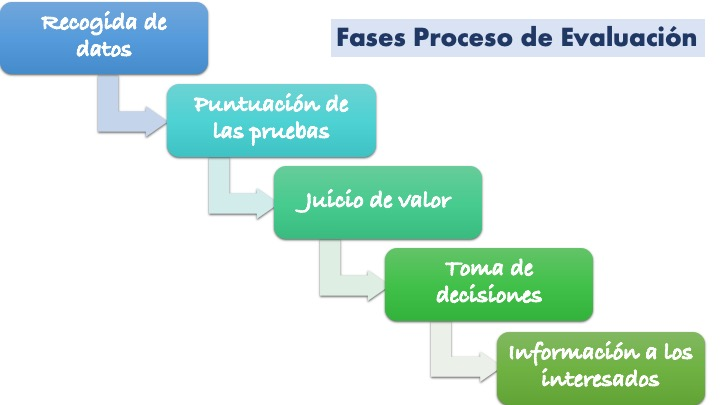
\includegraphics[width=0.6\linewidth]{imagen/fases-proceso-evaluacion.jpg}
 \caption{Fases en un proceso de evaluación}
 \label{fig:fases-evaluacion} 
\end{figure}

\subsection{Criterios de evaluación de un proceso}
Según la RAE (Real Academia Española), un criterio es una norma utilizada para conocer la verdad. Sin embargo, en cuanto a las evaluaciones, es un parámetro en función del que se juzgarán los atributos de un objeto de estudio \cite{RAE2022}. En este sentido, los criterios se construyen en función de lo que se desea obtener de un entrenamiento. Por lo general, son normas que se encuentran implícitas y permiten informar a los capacitados acerca del logro o fracaso de una determinada tarea. 

Pueden existir tantos criterios como parámetros se interpreten. Cada uno es el reflejo de un campo importante que se desea controlar. Por ejemplo: en los entrenamientos donde el tiempo influye en la evaluación, no sólo se mide la capacidad de aprendizaje del profesional, también se trata de evaluar la rapidez con la que reacciona, contando como parámetro importante para el desarrollo de la tarea. Este ejemplo se puede notar en el campo de la medicina \cite{Castrillon2021}.

\subsection{Proceso de validación de las respuestas}
Una vez terminada la capacitación se comprueban cuáles de los resultados obtenidos son correctos y cuáles no. Para ello se deben comparar las respuestas del evaluado con una fuente de confianza, que contenga la información verídica de lo que se está tratando. Estas fuentes de confianza se conocen por el nombre de: bases de conocimiento \cite{Rasheed2021}.

A partir de estas bases se verifica si los datos en las respuestas del evaluado coinciden con la información real contenida. Este proceso puede realizarse tanto de manera manual, semiautomática o automática.

%%%%%%%%%%%%%%%%%%%%%%%%%%%%%%%%%%%%%

\section{Sistemas de capacitación automatizados}
Teniendo en cuenta el concepto de capacitación, un sistema de capacitación automatizado es un método de enseñanza alternativo, creado para el adiestramiento de los trabajadores. Es un software que, principalmente, permite el aprendizaje de los usuarios sin necesidad de una supervisión constante. Por lo general, resulta más efectivo que las prácticas de enseñanza presencial, debido a que el estudiante trabaja solo y puede determinar su propia velocidad de aprendizaje, usando una amplia variedad de herramientas y métodos para la transferencia del conocimiento \cite{ISEM2022}.

A modo de resumen, es un programa informático que brinda una solución de recursos humanos, ayuda en la formación de los trabajadores y aumenta la productividad empresarial.

\subsection{Ventajas en un sistema de capacitación automatizado}
Un sistema de entrenamiento asistido por computadora, permite ofrecer el mismo nivel de adiestramiento para cada usuario del sistema, en cuanto a rigor y evaluación. Uno de los problemas principales de la capacitación de los empleados de manera presencial es que las sesiones son frecuentemente inconsistentes y las diferencias en el nivel de habilidad del formador pueden tener un impacto significativo en el éxito del empleado. Al contar con un sistema automatizado, solo se necesita una base de conocimiento para garantizar el mismo nivel de entrenamiento para todos. Por otra parte, una capacitación presencial requiere la existencia de una persona, por lo general un experto, que supervise al adiestrado y califique su rendimiento. En cambio, con estos sistemas, no es necesario desempeñar esta tarea, el propio software se encarga de la supervición y evaluación del capacitado \cite{Kanev2017}.

\subsection{Tipos de preguntas en un sistema de capacitación automatizado}
Con el paso del tiempo se generan nuevos métodos de estudio y con estos, nuevas formas de preguntas y calificaciones. Sin embargo, en el momento de diseñar un sistema automatizado, no es menos cierto que existen algunas variantes más sencillas y, por ende, más utilizadas. Según \cite{Laguna2016}, los tipos de preguntas que mayormente se emplean en los sistemas de capacitación automatizados son:

\begin{itemize}
\item \textbf{Verdadero o falso}: contienen una declaración que se debe indicar si es verdadera o no. Permiten responder en poco tiempo, son fáciles, rápidas de calificar y se corrigen de forma automática.
\item \textbf{Opción múltiple}: se componen de una pregunta (raíz) con múltiples respuestas posibles. Al poder incluir múltiples opciones válidas, podrían darse por superadas al marcar cualquiera de las respuestas o cuando se marquen todas. Se caracterizan por ser fáciles, rápidas de calificar, corregirse automáticamente y utilizarse para evaluar los conocimientos en una amplia gama de contenidos.
\item \textbf{Emparejar, relacionar u ordenar}: por lo general se emparejan cada una de las opciones del primer bloque con las opciones dadas en el segundo bloque, o se ordenan bloques de modo que quede una secuencia correcta de acuerdo a un patrón previamente establecido. Se suelen usar en aquellos cursos donde la adquisición de conocimientos muy detallados es un objetivo importante. Son preguntas fáciles de diseñar, rápidas de calificar y se corrigen automáticamente. Estadísticamente, se tarda más en responder este tipo de preguntas que las preguntas anteriores.
\item \textbf{Respuesta corta}: basta con que se escriban un par de palabras o una frase sencilla. Una alternativa más común a este tipo de preguntas es la de cubrir los espacios en blanco con una palabra. Son de gran utilidad a la hora de demostrar los conocimientos basados en hechos o palabras claves. La dificultad para calificarlas depende del estilo que se decida emplear.
\end{itemize}

\subsection{Colores utilizados en un sistema digital}
Se pudiese llegar a pensar que, en un sistema digital, los colores que se utilizan son totalmente aleatorios, pero esto es un error. Lo cierto es que unas tonalidades u otras provocan en el cerebro diferentes sensaciones que, aunque no se pueden percibir físicamente, influyen tanto en el estado de ánimo como en la productividad o creatividad. Sin embargo, no todos los colores tienen el mismo efecto en las personas, pero no es menos cierto que una gran mayoría comparten las mismas reacciones. De ahí la importancia de realizar un estudio detallado a la hora de seleccionar los tonos que representarán un sistema \cite{Paspuezan2022}.

\subsubsection{Psicología del color}
La psicología del color es un campo de estudio que está dirigido a analizar cómo se perciben y se reacciona ante distintos colores, así como las emociones que suscitan en las personas dichos tonos. El modo en el que los colores inducen a experimentar determinadas sensaciones y a adoptar ciertas actitudes tiene dos tipos de causas: las biológicas y las culturales. El área en la que más se aplica esta psicología es en el marketing \cite{Paspuezan2022}.

\subsubsection{Significado de los colores}
En el caso de un sistema digital, dependiendo del tipo de objetivo que se quiera conseguir, deberían ser los colores a utilizar. Cada color posee su propio significado y en \cite{TerronLopez2022} se comentan algunos:

\begin{itemize}
\item \textbf{Azul}: ayuda a mejorar la creatividad, estimula el pensamiento y la innovación, incita la resolución de problemas y trasmite paz. Mayormente se relaciona con entidades bancarias.
\item \textbf{Rojo}: mantiene la mente en estado de alerta, reduce la velocidad, permite recordar detalles y mejora la memoria.
\item \textbf{Amarillo}: es el color más llamativo, estimula el cerebro, representa el optimismo y trasmite energía y alegría. Las empresas lo utilizan para representar su creatividad y energía, aunque no debe usarse en exceso porque puede resultar molesto.
\item \textbf{Naranja}: activa la capacidad de aprendizaje, ayuda a la actividad mental y la concentración y mejora la creatividad y el análisis. Es un color muy utilizado en los sistemas de entrenamiento o en sistemas estudiantiles.
\item \textbf{Verde}: generalmente se asocia a la naturaleza, mejora las habilidades de lectura, ayuda a empatizar y fomentar ideas nuevas.
\end{itemize}

\subsubsection{Combinación de colores}
Para lograr una buena combinación de colores en un sistema se debe hacer uso de la gama cromática. Esta escala ordena los colores según su valor, saturación o posición. Se divide en cálida y fría (\textsl{Figura \ref{fig:colores}}). La gama cálida está integrada por colores que van desde el magenta hasta el amarillo verdoso (son tonos ideales para llamar la atención del usuario, siempre y cuando se usen con moderación). Los colores fríos van desde el púrpura al azul, y son utilizados con frecuencia por empresas que quieren representar seriedad y responsabilidad, pues transmiten calma a los usuarios \cite{TerronLopez2022} .

\begin{figure}[h]
\centering
 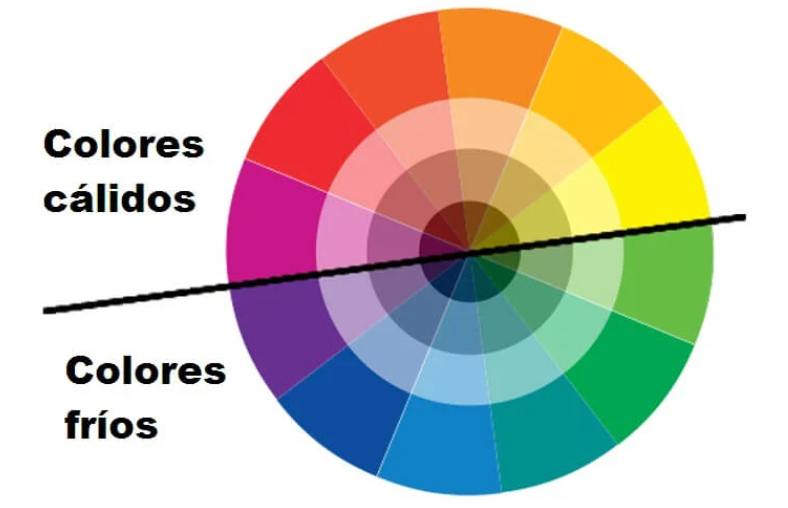
\includegraphics[width=0.6\linewidth]{imagen/gama.png}
 \caption{Gama cromática de colores (cálidos y fríos)}
 \label{fig:colores} 
\end{figure}

Una vez definidas las tonalidades se recomienda seguir un patrón de diseño para todo el sistema, basándose en: una gama cromática (diferentes tonos de un mismo color), una gama complementaria (un color combinado con sus complementarios) o una gama opuesta (un color combinado con el color opuesto) \cite{TerronLopez2022}.

\subsection{Proceso de validación de las respuestas}
En los sistemas de capacitación automatizados pueden emplearse tres métodos diferentes de validación: manual, semiautomático o automático. Por lo general, el más utilizado es el automático, porque facilita el trabajo para aquellos que deben diagnosticar a un personal abundante. Según \cite{AltyJames1984}, uno de los métodos más efectivos de evaluar las respuestas en un sistema es mediante el uso de sistemas expertos.

%%%%%%%%%%%%%%%%%%%%%%%%%%%%%%%%%%%%%

\section{Sistemas expertos}
Los sistemas expertos resuelven problemas que normalmente son solucionados por expertos humanos. Para hacerlo, necesitan acceder a una importante base de conocimiento sobre el dominio, que debe construirse de la manera más eficiente posible. Utilizan uno o más mecanismos de razonamiento, para aplicar este conocimiento a los problemas que se le proponen. Cuentan con un instrumento para explicar a los usuarios que han confiado en ellos, lo que han hecho y cómo \cite{VonRueden2021}.

Una forma de contemplar estos sistemas es que simbolizan la mayor parte de la Inteligencia Artificial (IA) aplicada. Un sistema experto en IA se define como un programa informático que tiene la capacidad de representar y razonar sobre el conocimiento \cite{Rasheed2021}.

\subsection{Desventajas de los sistemas expertos}
Al ser una tecnología novedosa, los sistemas expertos traen consigo ciertas desventajas. Por presentar algunos ejemplos, en \cite{Kandula2020} se mencionan:

\begin{itemize}
\item Su actualización necesita de reprogramación, siendo una de sus limitaciones más acentuadas
\item Son poco flexibles a cambios y de difícil acceso a información no estructurada
\item Poseen un elevado costo monetario y de tiempo
\item Carecen de sentido común (no hay nada obvio)
\item No se puede mantener una conversación informal con ellos
\item Es muy complicado que aprendan de sus errores o de errores ajenos
\item No son capaces de distinguir cuáles son las cuestiones relevantes de un
problema y separarlas de cuestiones secundarias
\end{itemize}

Sin embargo, estos problemas no solo los presentan los sistemas expertos. La IA aún no ha podido desarrollar sistemas que
sean capaces de aplicar el sentido común humano para resolver situaciones complejas. Es por ello que, a pesar de sus desventajas, los sistemas expertos son considerados una gran ayuda y un enorme avance, en especial, en el campo de los sistemas de capacitación \cite{Barham2022}.

\subsection{Ventajas de los sistemas expertos}
El uso de un sistema experto en cualquier ámbito social resulta favorable de diversas maneras. Según \cite{Mitchell1990}, entre sus ventajas más notables se pueden encontrar:

\begin{itemize}
\item No sufre de limitaciones y percances humanos, lo que lo convierte en una herramienta estable y fiable para su entorno
\item Sus actividades son completamente replicables y siempre contesta de la misma manera a menos que se le cambie el diseño
\item La velocidad de procesamiento es mayor a la de un ser humano
\item Pueden almacenar su conocimiento para cuando sea necesario aplicarlo
\item Pueden ser utilizados por personas no especializadas para resolver problemas
\item Pueden ser usados como sistema de aprendizaje
\item Al evaluar el costo total del empleo de esta tecnología, la replicabilidad y estabilidad, asociado a la seguridad que provee, resulta una ecuación favorable, aún considerando que las inversiones iniciales pueden ser
relativamente elevadas
\end{itemize}

A modo de conclusión, dependiendo del ámbito y los objetivos que se persigan, por lo general, el uso de esta tecnología representa un avance más que una desventaja.

\subsection{Componentes de un sistema experto}
En \cite{Omuya2021} se detallan los diferentes componentes que integran un sistema experto. Aunque pueden contar con un número mayor, los mínimos requeridos son (\textsl{Figura \ref{fig:componentes}}):

\begin{itemize}
\item \textbf{Motor de inferencia}: es el corazón del sistema experto. Su cometido principal es sacar conclusiones aplicando el conocimiento a los datos. Estas conclusiones pueden estar basadas en conocimiento determinista o probabilístico.
\item \textbf{Base de conocimiento}: consiste en un conjunto de objetos y un conjunto de reglas que gobiernan las relaciones entre ellos. La información que almacena es de naturaleza permanente y estática, es decir, no cambia de una aplicación a otra. Se debe diferenciar entre los datos y el conocimiento. Con conocimiento se refiere: a las afirmaciones de validez general, tales como reglas, distribuciones de probabilidad, entre otras. Con datos se refiere: a la información que se tiene de una aplicación en particular.
\item \textbf{Mecanismo de aprendizaje}: controla el flujo de información que va del experto humano a la base de conocimiento. El sistema determina qué nueva información se necesita, o si los datos son reales, es decir, si debe incluirse nuevo conocimiento, y en caso necesario incorporarlo.
\item \textbf{Interfaz de usuario}: es la interfaz entre el sistema experto y el usuario. Para que sea efectiva debe incorporar mecanismos para mostrar y obtener información de forma sencilla y agradable.
\end{itemize}

\begin{figure}[h]
\centering
 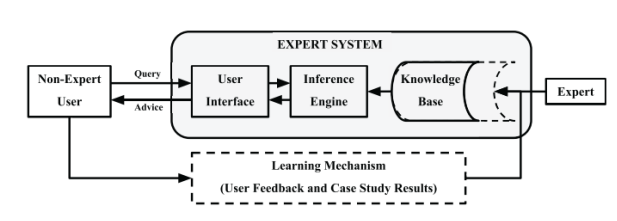
\includegraphics[width=0.7\linewidth]{imagen/componentes.png}
 \caption{Componentes de un sistema experto}
 \label{fig:componentes} 
\end{figure}

%%%%%%%%%%%%%%%%%%%%%%%%%%%%%%%%%%%%%%%%

\section{Sistema Generador de Bases de Conocimiento}
En octubre del 2017, el Instituto de Investigaciones de la Industria Alimentaria (IIIA), en conjunto con las facultades de Ingeniería Química e Ingeniería Informática de la Universidad Tecnológica de La Habana José Antonio Echeverría (CUJAE), desarrolló un Sistema Gestor de Bases de Conocimiento (SGBC). La función principal de este sistema es generar bases de información a partir de los datos introducidos por un usuario determinado. Dichas bases son exportadas en dos tipos especiales de ficheros: \textsl{anm} y \textsl{drl}. Cada uno de estos ficheros contienen información sobre un proceso productivo determinado \cite{Lemus2018}.

\subsection{Funcionamiento del generador}
El generador tiene como objetivo crear bases de conocimiento sobre procesos productivos industriales. Utiliza reglas de producción como formalismo de representación del conocimiento, las cuales se generan según el formato definido por el motor de inferencia \textsl{Drools}.

En el SGBC todos los datos son introducidos por un usuario, que puede crear o cargar un proceso productivo de cualquier rama de la Industria Alimentaria. Por cada proceso se deben incluir las diferentes variables que en este influyen e ir clasificándolas en tres tipos: discretas, válvulas o continuas. En el caso de ser continuas se les deben agregan sus valores máximos y mínimos. Una vez introducidas todas las variables, se empiezan a insertar las causas que influyen sobre las mismas y, luego, las recomendaciones para cada una de ellas, aunque el orden de los datos no afecta el resultado. Solo al concluir, se podrán emparejar cada variable con sus causas y, cada causa, con sus recomendaciones. Se debe tener en cuenta que una variable puede vincularse a varias causas y que una causa puede necesitar varias recomendaciones. Al emparejar una variable con su causa se debe indicar el estado en el que se encuentra: si es discreta puede ser positivo o negativo; si es válvula puede ser abierto, normal o cerrado y si es continua puede ser alto, normal o bajo. Una vez concluida la entrada de los datos, la información se exporta en los ficheros \textsl{anm} y \textsl{drl} \cite{Riveron2017}.

\subsection{Información de los ficheros anm}
Un archivo \textsl{anm} puede ser utilizado por diferentes tipos de programas distribuidos, para múltiples plataformas como Linux, Mac o Windows. En este caso, estos ficheros contienen toda la información referente a las variables, causas y recomendaciones de un proceso productivo.
Comienzan con los nombres de las variables y su clasificación. Si la variable es de tipo continua, poseen sus valores máximos y mínimos. Cada información de las variables está separada por comas, y cada variable está dividida por renglones.
Al finalizar, aparece un indicador (*causa) que representa el inicio de un nuevo bloque de información: las causas. Las causas solo poseen su nombre y están separadas por renglones. Finalizando ese bloque, aparece otro indicador (*recomendaciones) para representar el inicio del último bloque de información: las recomendaciones.
De las recomendaciones solo se tiene el nombre y cada una está separada por renglones. Con el último indicador (-1), se da a entender que se finalizó la información del fichero \cite{Riveron2017}.

\subsection{Información de los ficheros drl}
Un archivo \textsl{drl} es donde el motor de inferencia \textsl{Drools} (Sistema de Gestión de Reglas de Negocio en español) almacena sus reglas (\textsl{Figura \ref{fig:reglas}}). La estructura de una regla dentro de este archivo sigue un patrón determinado, donde \textbf{name} es el nombre de la regla, \textbf{attribute} son los posibles atributos que puede tener, \textbf{conditional element} es la sentencia condicional a evaluar y, si se cumple esta sentencia, se realizan una o varias acciones en \textbf{action}. En este caso, lo que se almacenan son  las reglas entre variables y causas y entre causas y recomendaciones \cite{Riveron2017}.

\begin{figure}[h]
\centering
 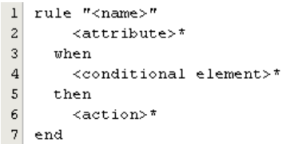
\includegraphics[width=0.47\linewidth]{imagen/rules.png}
 \caption{Estructura del fichero \textsl{drl} (reglas)}
 \label{fig:reglas} 
\end{figure}

%%%%%%%%%%%%%%%%%%%%%%%%%%%%%%%%%%%%%%%%

\section{Sistema de entrenamiento SECPROIT}
En el año 2018 se creó el Sistema Experto para el Control de Procesos Químicos (SECPROIT), diseñado para capacitar a los operarios de la Industria Alimentaria Cubana sobre los diferentes procesos productivos que en ella se realizan. Este sistema fue desarrollado en la Universidad Tecnológica de La Habana José Antonio Echeverría (CUJAE), entre las facultades de Ingeniería Química e Ingeniería Informática. Su objetivo principal era lograr capacitar a los operarios de la industria y, para ello, realizar un conjunto de entrenamientos evaluados por un sistema experto \cite{ElenaAcostaGil2018}.

\subsection{Funcionamiento del SECPROIT}
El sistema está diseñado para capacitar a los trabajadores de las fábricas a partir de entrenamientos relacionados a los procesos productivos que en ellas se realizan, mediante el uso de un sistema experto. En el sistema, existen tres roles fundamentales: 

\begin{itemize}
\item Administrador: se encarga del control de los datos del sistema
\item Especialista: es el responsable de insertar las bases de conocimiento y supervisa los resultados obtenidos por los trabajadores de su área laboral
\item Operario: realiza los entrenamientos
\end{itemize}

Cada usuario posee un nombre, una contraseña y un rol, y con cada rol aparecen funcionalidades únicas y específicas. En el caso de los especialistas, para insertar una base de conocimiento deben asociarla a un proceso, y de cada proceso deben registrar el nombre, una imagen (si la posee), un fichero tipo \textsl{anm} y un archivo \textsl{drl}. El operario entrará a realizar aquellos entrenamientos que el especialista haya validado \cite{Lemus2018}.

Una vez comenzada la prueba, el usuario deberá señalar de un grupo de variables las que por su estado estén en peligro de inestabilidad. Si ha seleccionado correctamente pasa a la siguiente etapa, donde debe escoger qué causa el estado de las variables que prefirió. Por último, deberá seleccionar qué recomendaciones seguir para cada causa señalada \cite{ElenaAcostaGil2018}.

El SECPROIT posee un grupo de reportes que facilita la toma de decisiones a partir de los resultados alcanzados. El especialista puede contar con una lista de resultados de cada operario de su área y, de esta forma, se garantiza la selección de los mejores trabajadores a partir de la organización brindada por la lista. También se puede encontrar un listado de los cambios realizados en el sistema, junto con la fecha y el nombre del usuario que los realizó. Este último reporte colabora con la seguridad.

\subsection{Limitaciones actuales del sistema}
Actualmente el sistema SECPROIT posee ciertas limitaciones que impiden que sea implementado en las industrias:
\begin{itemize}
\item Cada vez que se desea utilizar la información obtenida por el generador es extraída directamente desde sus ficheros, lo que genera una demora extra en el sistema
\item Solo existe un modelo de pregunta, por lo que resulta redundante el método de evaluación
\item El tiempo demorado en responder el entrenamiento no influye en la nota final del mismo
\item La etapa de las recomendaciones no se evalúa
\item Las etapas aparecen de forma continúa, sin oportunidad de una pausa
\item Aparecen todas las etapas en una misma vista, si se suspende una, se muestran etapas innecesariamente
\item Por cada proceso existe un único entrenamiento
\item Presenta una interfaz gráfica poco vistosas y de colores muy oscuros que generan desagrado en los usuarios
\end{itemize}

%%%%%%%%%%%%%%%%%%%%%%%%%%%%%%%%%%%%%%%%

\section{Conclusiones parciales}
Al concluir el capítulo se puede arribar a las siguientes conclusiones:
\begin{itemize}
\item La capacitación constante de los trabajadores de una empresa ayuda al rendimiento de la misma y evita errores futuros
\item Los sistemas de capacitación automatizados permiten el entrenamiento del personal laboral sin la necesidad de un supervisor, lo que ahorra tiempo y recursos humanos a la empresa
\item En un sistema de capacitación automatizado se pueden medir tantos parámetros de aprendizaje como herramientas se tenga
\item Los criterios de evaluación de un entrenamiento varían según los parámetros y requisitos de la empresa
\item En los sistemas digitales, el color naranja aumenta la concentración y el nivel de aprendizaje, por lo que este color es muy utilizado en los sistemas de entrenamiento y en sistemas estudiantiles
\item Los sistemas expertos facilitan el proceso de evaluación de los sistemas de entrenamiento digitales
\item El SGBC genera las bases de conocimiento del sistema SECPROIT y puede ser utilizado para cualquier tipo de proceso productivo dentro de la Industria Alimentaria Cubana
\item El sistema SECPROIT posee un conjunto de limitaciones que impiden su completo funcionamiento
\end{itemize}